\documentclass[
11pt, % The default document font size, options: 10pt, 11pt, 12pt
codirector, % Uncomment to add a codirector to the title page
]{charter} 




% El títulos de la memoria, se usa en la carátula y se puede usar el cualquier lugar del documento con el comando \ttitle
\titulo{Detector automático de objetos para despensa inteligente} 

% Nombre del posgrado, se usa en la carátula y se puede usar el cualquier lugar del documento con el comando \degreename
\posgrado{Carrera de Especialización en Sistemas Embebidos} 
%\posgrado{Carrera de Especialización en Internet de las Cosas} 
%\posgrado{Carrera de Especialización en Intelegencia Artificial}
%\posgrado{Maestría en Sistemas Embebidos} 
%\posgrado{Maestría en Internet de las cosas}

% Tu nombre, se puede usar el cualquier lugar del documento con el comando \authorname
\autor{Ing. Santiago Andrés Bualó} 

% El nombre del director y co-director, se puede usar el cualquier lugar del documento con el comando \supname y \cosupname y \pertesupname y \pertecosupname
\director{Mgs. Ing. Matías Brignone}
\pertenenciaDirector{pertenencia} 
% FIXME:NO IMPLEMENTADO EL CODIRECTOR ni su pertenencia
\codirector{John Doe} % para que aparezca en la portada se debe descomentar la opción codirector en el documentclass
\pertenenciaCoDirector{FIUBA}

% Nombre del cliente, quien va a aprobar los resultados del proyecto, se puede usar con el comando \clientename y \empclientename
\cliente{-}
\empresaCliente{-}

% Nombre y pertenencia de los jurados, se pueden usar el cualquier lugar del documento con el comando \jurunoname, \jurdosname y \jurtresname y \perteunoname, \pertedosname y \pertetresname.
\juradoUno{Nombre y Apellido (1)}
\pertenenciaJurUno{pertenencia (1)} 
\juradoDos{Nombre y Apellido (2)}
\pertenenciaJurDos{pertenencia (2)}
\juradoTres{Nombre y Apellido (3)}
\pertenenciaJurTres{pertenencia (3)}
 
\fechaINICIO{1 de septiembre de 2023}		%Fecha de inicio de la cursada de GdP \fechaInicioName
\fechaFINALPlan{1 de octubre de 2023} 	%Fecha de final de cursada de GdP
\fechaFINALTrabajo{15 de marzo de 2024}	%Fecha de defensa pública del trabajo final


\begin{document}

\maketitle
\thispagestyle{empty}
\pagebreak


\thispagestyle{empty}
{\setlength{\parskip}{0pt}
\tableofcontents{}
}
\pagebreak


\section*{Registros de cambios}
\label{sec:registro}


\begin{table}[ht]
\label{tab:registro}
\centering
\begin{tabularx}{\linewidth}{@{}|c|X|c|@{}}
\hline
\rowcolor[HTML]{C0C0C0} 
Revisión & \multicolumn{1}{c|}{\cellcolor[HTML]{C0C0C0}Detalles de los cambios realizados} & Fecha      \\ \hline
0      & Creación del documento                                 &\fechaInicioName \\ \hline
1      & Primera entrega                                  & 3 de septiembre de 2023 \\ \hline
2      & Segunda entrega                                   &10 de septiembre de 2023\\ \hline
1      & Tercera entrega                                  & 20 de septiembre de 2023 \\ \hline
%1      & Se completa hasta el punto 4 inclusive                 & dd/mm/aaaa \\ \hline
%2      & Se completa hasta el punto 7 inclusive
%		  Se puede agregar algo más \newline
%		  En distintas líneas \newline
%		  Así                                                    & dd/mm/aaaa \\ \hline
%3      & Se completa hasta el punto 11 inclusive                & dd/mm/aaaa \\ \hline
%4      & Se completa el plan	                                 & dd/mm/aaaa \\ \hline
\end{tabularx}
\end{table}

\pagebreak



\section*{Acta de constitución del proyecto}
\label{sec:acta}

\begin{flushright}
Buenos Aires, \fechaInicioName
\end{flushright}

\vspace{2cm}

Por medio de la presente se acuerda con el \authorname\hspace{1px} que su Trabajo Final de la \degreename\hspace{1px} se titulará ``\ttitle'', consistirá esencialmente en la implementación de un prototipo de un sistema de alacena inteligente capaz de mantener un inventario de los objetos dentro de la misma, detectando los productos que ingresan y egresan en tiempo real, y tendrá un presupuesto preliminar estimado de 620 h de trabajo y \textcolor{red}{\$XXX}, con fecha de inicio \fechaInicioName\hspace{1px} y fecha de presentación pública \fechaFinalName.

Se adjunta a esta acta la planificación inicial.

\vfill

% Esta parte se construye sola con la información que hayan cargado en el preámbulo del documento y no debe modificarla
\begin{table}[ht]
\centering
\begin{tabular}{ccc}
\begin{tabular}[c]{@{}c@{}}Dr. Ing. Ariel Lutenberg \\ Director posgrado FIUBA\end{tabular} & \hspace{2cm} \vspace{2.5cm} \\ 
\multicolumn{3}{c}{\begin{tabular}[c]{@{}c@{}} \supname \\ Director del Trabajo Final\end{tabular}} \vspace{2.5cm} \\
%\begin{tabular}[c]{@{}c@{}}\jurunoname \\ Jurado del Trabajo Final\end{tabular}     &  & \begin{tabular}[c]{@{}c@{}}\jurdosname\\ Jurado del Trabajo Final\end{tabular}  \vspace{2.5cm}  \\
%\multicolumn{3}{c}{\begin{tabular}[c]{@{}c@{}} \jurtresname\\ Jurado del Trabajo Final\end{tabular}} \vspace{.5cm}                                                                     
\end{tabular}
\end{table}




\section{1. Descripción técnica-conceptual del proyecto a realizar}
\label{sec:descripcion}



El presente trabajo práctico busca implementar un sistema de alacena inteligente, el cual pueda mantener un inventario de los objetos dentro de la misma de forma autónoma y automática, mediante la detección de los productos que ingresan y/o egresan a la despensa en tiempo real, en el instante en que se agregan o se remueven.

Se ha observado que  una de las problemáticas más frecuentes en el marco de las compras cotidianas para el hogar, es que las personas muestran una tendencia a olvidarse de las cosas que deben comprar. El objetivo principal de este proyecto es solventar esta problemática aplicando un método que la industria viene aplicando hace ya varios años: control de inventario. Esto será realizado de forma automática mediante un conjunto de sensores capaces de detectar los objetos que ingresan o egresan a la despensa, de forma tal de poder llevar a cabo un conteo de los objetos presentes o faltantes, permitiendo tener siempre a mano el estado de la despensa (o alacena), lo que supondrá una mejora en la gestión de las cosas que se tienen en el hogar. También permitirá entender las necesidades de consumo diario, semanal, quincenal o mensual de los distintos productos presentes en el hogar, lo que facilitará la creación de listas de supermercado de forma periódica y automática. Además, se podrá consultar este estado desde cualquier lugar, mediante el acceso desde una aplicación. 

A día de hoy las grandes industrias están implementando mejoras y soluciones en los hogares de forma constante, tratando de modernizar todos los electrodomésticos, ambientes y elementos. Sin embargo, si se observa problemática planteada, en las soluciones propuestas hasta la fecha, no existen soluciones que aborden esta problemática de forma clara, concisa y , por sobre todo, útil para la sociedad. En particular, hasta la fecha, lo más parecido a lo que se ha planteado, consta de una solución propuesta por Samsung: ha integrado a sus heladeras una aplicación que lleva un inventariado de la misma, pero de forma manual, siendo el usuario quien ingresa a mano qué objetos ingresan, y qué objetos utilizan o extraen.

La propuesta planea no solo superar con creces la oferta actual del mercado, buscando subsanar la problemática desde la raíz, sino que también tiene como objetivo el sentar precedentes para ser el principio de numerosos avances en cuanto a esta tecnología, los que continúen mejorando la calidad de vida de las personas, impulsando un nuevo paradigma. 

Este nuevo paradigma, consiste en rediseñar las alacenas, incorporando tecnología del siglo XXI. El concepto de inventario ya está más que establecido en  industrias y empresas, las que se ven altamente beneficiadas en productividad gracias al ahorro de tiempo que  conlleva entender no solo la distribución de los objetos, sino también cuando es necesario reponerlos. Ese mismo beneficio es el que se va a estar trasladando a los hogares. Con esta nueva gestión de inventario en las alacenas, se pueden automatizar un sinfín de procesos y tomas de decisiones propias del hogar que quitan tiempo personal. Este inventario automático, va a permitir mejoras en los siguientes aspectos:

\begin{itemize}
    \item Entender los consumos del hogar de los distintos productos.
    \item Interpretar los tiempos de reposición de cada producto, lo que permite generar listas de compra para diferentes períodos.
    \item Conocer qué productos se tienen en tiempo real, permitiendo tomar decisiones sobre los menús para las siguientes comidas.
\end{itemize}

Para llevar a cabo este proyecto, se propone un módulo integral capaz de detectar el ingreso/egreso de los productos hacia la despensa, computar la cantidad de productos y mantener el inventario dentro de si mismo. Además, deberá tener la capacidad para comunicarse con la red, no solo para posibilitar detectar un mayor número de elementos, sino también para poder llevar a cabo un respaldo del inventario interno, de forma tal de poder disponibilizarlo al usuario desde otra interfaz (por ejemplo web o aplicación móvil). 
Todo va a estar orquestado por un núcleo de procesamiento (microcontrolador), el cual se comunicará con un lector de código de barras para detectar al producto. Luego, mediante llamados de API, se va a identificar al producto, y se va a proceder a realizar el cómputo para modificar el inventario.
El dispositivo deberá ser alimentado mediante una batería, ya sea desechable o recargable, de forma tal de independizar al usuario sobre la posición en la cual debe instalar al producto.
A continuación se puede ver en la figura \ref{fig:diagBloques} un diagrama de bloques sobre el prototipo:

\begin{figure}[htpb]
\centering 
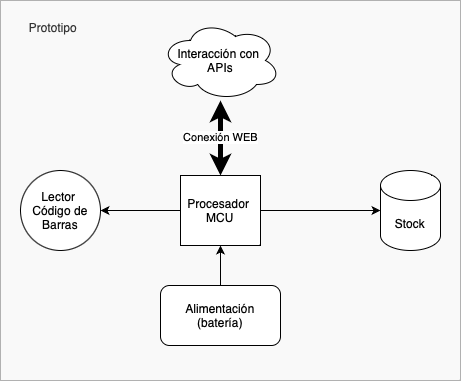
\includegraphics[width=.75\textwidth]{./Figuras/DiagramaBloque.png}
\caption{Diagrama en bloques del sistema propuesto.}
\label{fig:diagBloques}
\end{figure}

\vspace{25px}

\newpage

\section{2. Identificación y análisis de los interesados}
\label{sec:interesados}

A continuación se listan a todas las partes involucradas al proyecto:

\begin{table}[ht]
%\caption{Identificación de los interesados}
%\label{tab:interesados}
\begin{tabularx}{\linewidth}{@{}|l|X|X|l|@{}}
\hline
\rowcolor[HTML]{C0C0C0} 
Rol           & Nombre y Apellido & Organización 	& Puesto 	\\ \hline
Auspiciante   &           \authorname         &          -    	&        	\\ \hline
Responsable   & \authorname       & FIUBA        	& Alumno 	\\ \hline
Orientador    & \supname	      & \pertesupname 	& Director Trabajo final \\ \hline
Usuario final &  Acreedores de alacena                 &              	&        	\\ \hline
\end{tabularx}
\end{table}


\begin{itemize}
	\item Auspiciante: siendo un proyecto personal, todos los gastos y/o beneficios serán incurridos por el autor del proyecto.
	\item Responsable: \authorname, quien va a ser el responsable del proyecto, siendo el autor del mismo.
 	\item Usuario final: como el proyecto esta orientado como solución para los hogares, el usuario final serán todas aquellas personas dueñas de una alacena.
 
\end{itemize}



\section{3. Propósito del proyecto}
\label{sec:proposito}

El propósito de este proyecto es impulsar nuevas tecnologías dentro del hogar mediante la modernización de uno de los lugares que más se utiliza dentro del mismo, posibilitando una mejor gestión de los distintos productos que se guardan dentro. Gracias a esta nueva metodología se busca que los usuarios encuentren una nueva forma mucho más sencilla y eficiente de la toma de decisiones en las compras cotidianas.

\section{4. Alcance del proyecto}
\label{sec:alcance}

En el proyecto se incluye :

\begin{itemize}
	\item El desarrollo de un dispositivo que detecta el ingreso y egreso de objetos.
	\item Es desarrollo del dispositivo debe tener la capacidad para detectar de qué objeto se trata mediante la lectura del código de barras y luego llevar a cabo el conteo relacionadas al inventario.
 	\item El desarrollo de una interfaz externa al dispositivo que permita consultar el estado del inventario.
  \item El desarrollo de un menú de configuración rápida para el dispositivo.
  \item El desarrollo de una placa integrada como prototipo.
  \item La configuración de red para que el dispositivo pueda utilizar APIs para consultar el código de barras.
  \item El sistema de alimentación propio del prototipo.
  
\end{itemize}

No serán parte del proyecto los siguientes:

\begin{itemize}
	\item No se desarrollará un producto final para ser comercializado.
	\item No se contemplará almacenamiento externo o almacenamiento en la nube.
  
\end{itemize}

\section{5. Supuestos del proyecto}
\label{sec:supuestos}


Para el desarrollo del presente proyecto se supone que:

\begin{itemize}
	\item El dinero disponible será suficiente para la adquisición de los materiales requeridos.
	\item Se presume que todos los componentes originales con los que es planteado el proyecto tendrán stock.
 \item Todos los componentes se consiguen de forma local sin ningún impedimento.
  
\end{itemize}

\newpage

\section{6. Requerimientos}
\label{sec:requerimientos}


A continuación se enumerarán los requerimientos del proyecto:

\begin{enumerate}
	\item Requerimientos generales del sistema
		\begin{enumerate}
			\item El sistema debe detectar cuándo se ingresa o se egresa un objeto de la despensa.
			\item El sistema debe tener la capacidad de identificar de qué objeto se trata.
			\item El sistema debe llevar a cabo un conteo de los objetos que ingresan y/o egresan.
    \item El sistema debe almacenar el inventario de forma local.
    \item El sistema debe tener una aplicación web/móvil para poder consultar el inventario en tiempo real.
           
		\end{enumerate}
	\item Requerimientos de hardware
		\begin{enumerate}
			 \item El módulo deberá alimentarse a través de una batería.
			\item El módulo deberá poder comunicarse utilizando el estándar IEEE 802.11 b/g/n
(Wi-Fi).
            \item El módulo deberá poder comunicarse utilizando Bluetooth Low Energy (BLE).
            \item El módulo utilizará un único chip que integre el microprocesador y la conectividad Wi-Fi/Bluetooth.
            \item El módulo deberá comunicarse vía API a la red para identificar el producto.
            \item El módulo deberá detectar los códigos de barras mediante un lector apropiado o cámara fotográfica.
		\end{enumerate}
	\item Requerimientos de firmware
         \begin{enumerate}
            \item El firmware del módulo deberá ser programado en lenguaje C.
            \item Se realizarán tests de forma independiente para cada módulo, y de integración para cada una de las funcionalidades del mismo.
            \item El firmware deberá priorizar el ahorro energético. 
         \end{enumerate}
	\item Requerimientos de gestión
        \begin{enumerate}
            \item Se utilizará un repositorio público en Github como sistema de control de versiones.
         \end{enumerate}
    \item Requerimientos de documentación
        \begin{enumerate}
            \item Se escribirá un informe de avance de trabajo.
            \item Se escribirá una memoria de trabajo final.

            
         \end{enumerate}

    
	
\end{enumerate}

\section{7. Historias de usuarios (\textit{Product backlog})}
\label{sec:backlog}

En esta sección se enuncian las historias de usuario, asignándoles a cada una un puntaje según los siguientes aspectos:
    \begin{enumerate}
        \item Dificultad de la tarea/trabajo.
        \item Complejidad del trabajo.
        \item Riesgo asociado.
    \end{enumerate}

Para asignarles la ponderación, se utilizará una escala siguiendo la serie de Fibonacci, para lo cual un número mayor implica un mayor costo. Para calcular el Story Point, se sumarán las tres ponderaciones asignadas, y en caso de que el resultado no pertenezca a la serie, se le asignará el número superior más cercano.

\begin{enumerate}
    \item Como usuario quiero instalar el producto de forma sencilla para poder colocarlo en el lugar que me resulte más útil y menos molesto.
        \begin{itemize}
            \item Dificultad: 5
            \item Complejidad: 5
            \item Riesgo: 8
            \item Story Point: 21
        \end{itemize}

     \item Como usuario no quiero estar pendiente de cambiar/recargar la batería para estar constantemente pendiente de su remanente.
        \begin{itemize}
            \item Dificultad: 13
            \item Complejidad: 13
            \item Riesgo: 3
            \item Story Point: 34
        \end{itemize}

    \item Como usuario quiero una interfaz de usuario sencilla para que me resulte fácil de aprender y fácil de usar.
        \begin{itemize}
            \item Dificultad: 2
            \item Complejidad: 3
            \item Riesgo: 5
            \item Story Point: 13
        \end{itemize}

    \item Como usuario quiero consultar mi inventario en todo momento para determinar qué debo comprar.
        \begin{itemize}
            \item Dificultad: 3
            \item Complejidad: 8
            \item Riesgo: 2
            \item Story Point: 13
        \end{itemize}
    \item Como usuario quiero que el producto sea lo más pequeño posible para que no me quite lugar de almacenamiento.
        \begin{itemize}
            \item Dificultad: 13
            \item Complejidad: 8
            \item Riesgo: 5
            \item Story Point: 34
        \end{itemize}
\end{enumerate}

\section{8. Entregables principales del proyecto}
\label{sec:entregables}


Los entregables del proyecto son:

\begin{itemize}
	\item Diagrama de circuitos esquemáticos.
	\item Código fuente del programa.
	\item Guía de usuario.
	\item Diagrama PCB.
	\item Archivos de fabricación.
\end{itemize}


\section{9. Desglose del trabajo en tareas}
\label{sec:wbs}

A continuación se listan las tareas, junto con su duración es (en horas de trabajo):

\begin{enumerate}
\item Planificación y gestión del proyecto (90 h):
	\begin{enumerate}
	\item Realizar un plan de trabajo (20 h)
	\item Determinar componentes (10 h)
    \item Planificar la programación del firmware (20 h)
	\item Redactar informes y presentaciones (30 h)
    \item Redactar guía de usuario y otros documentos afines (10 h)
	\end{enumerate}
\item Investigación previa (125 h)
	\begin{enumerate}
	\item Investigar soluciones propuestas similares (20 h)
	\item Investigar microcontroladores (10 h)
	\item Investigar componentes periféricos afines (20 h)
    \item Investigar el estándar de código de barras (10 h)
    \item Investigar métodos de lectura de códigos de barra (30 h)
    \item Investigar bibliotecas y APIs afines (15 h)
    \item Investigar protocolos Wi-Fi y BLE (20 h)
	\end{enumerate}
\item Desarrollo de software (130 h)
	\begin{enumerate}
	\item Desarrollo de drivers específicos para cada periférico (25 h)
	\item Integración de drivers y bibliotecas (15 h)
	\item Elaborar la máquina de estados para el flujo del programa (10 h)
	\item Desarrollo de la interfaz de usuario (30 h)
    \item Implementación de FreeRTOS y Low Power Consumption (30 h)
    \item Optimización del código (20 h)
	\end{enumerate}
 \item Desarrollo de hardware (145 h)
	\begin{enumerate}
	\item Elección del microcontrolador (5 h)
	\item Elección del sensor de código de barras (5 h)
    \item Elección de integrados para los módulos Wi-Fi y BLE (10 h)
	\item Ensamblado del prototipo funcional (5 h)
	\item Diseño del circuito electrónico final (30 h)
    \item Diseño del PCB final (30 h)
    \item Generar archivos de fabricación (40 h)
    \item Optimización (20 h)
	\end{enumerate}
 \item Fabricación del prototipo (60 h)
	\begin{enumerate}
	\item Fabricado de la placa (10 h)
	\item Compra de componentes (5 h)
	\item Ensamblado de componentes (15 h)
	\item Diseño y fabricación de la caja (30 h)
	\end{enumerate}
  \item Pruebas, ensayos y validaciones (70 h)
	\begin{enumerate}
	\item Ensayos de señales eléctricas (10 h)
	\item Pruebas de comunicaciones Wi-Fi y BLE (10 h)
	\item Pruebas generales de integración (20 h)
	\end{enumerate}
\end{enumerate}

Cantidad total de horas: (620 h)

\section{10. Diagrama de Activity On Node}
\label{sec:AoN}

A continuación se muestra el diagrama de Activity on Node correspondiente con las tareas enunciadas en la sección anterior.

\begin{figure}[htpb]
\centering 
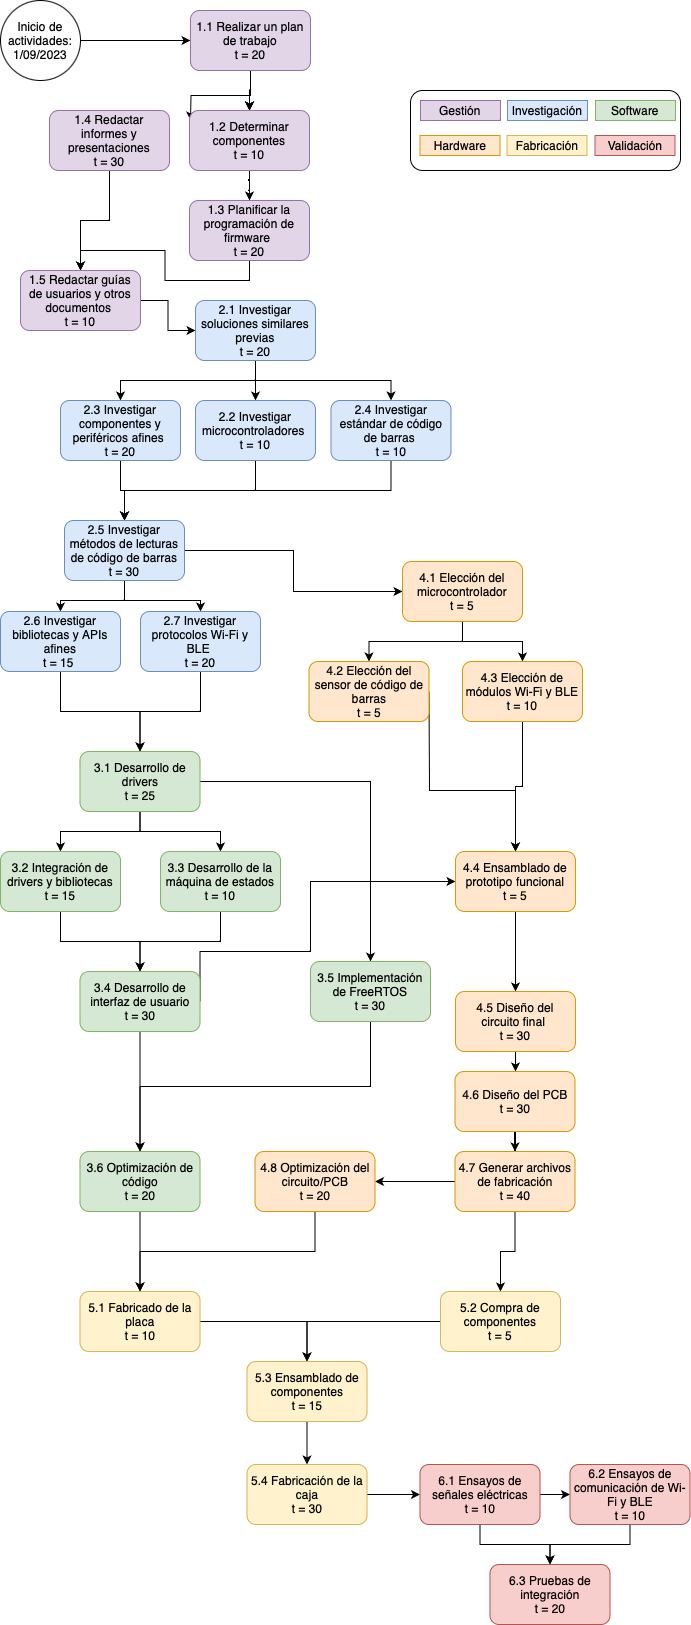
\includegraphics[width=.6\textwidth]{./Figuras/diagramaAoN.png}
\caption{Diagrama de \textit{Activity on Node}.}
\label{fig:AoN}
\end{figure}

Todos los tiempos indicados están expresados en horas, y se puede observar un camino crítico de las tareas 1.1, 1.4,1.5,2.1,2.3,2.5,4.1,4.3,4.4,4.5,4.6,4.7,4.8,5.1,5.3,5.4,6.1,6.2,6.3



\section{11. Diagrama de Gantt}
\label{sec:gantt}

A continuación se muestra la lista de tareas utilizada para realizar el diagrama de Gantt. Se consideró una semana de trabajo de 5 días, entendiendo que los días sábado y domingo no son laborables.
\begin{figure}[htpb]
\centering 
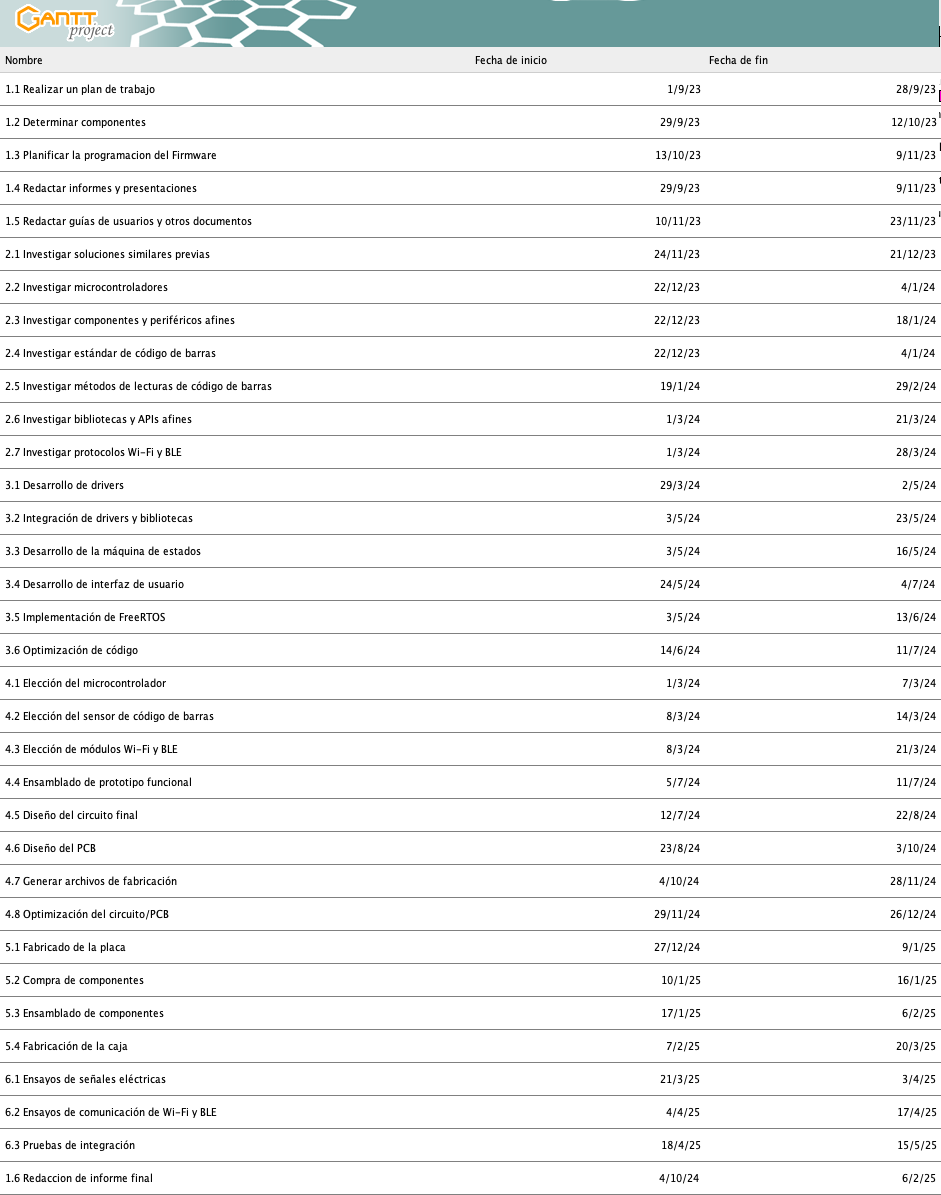
\includegraphics[width=\textwidth]{./Figuras/Lista.png}
\caption{Diagrama del \textit{Listado de tareas}.}
\label{fig:AoN}
\end{figure}


\begin{landscape}
\begin{figure}[htpb]
\centering 
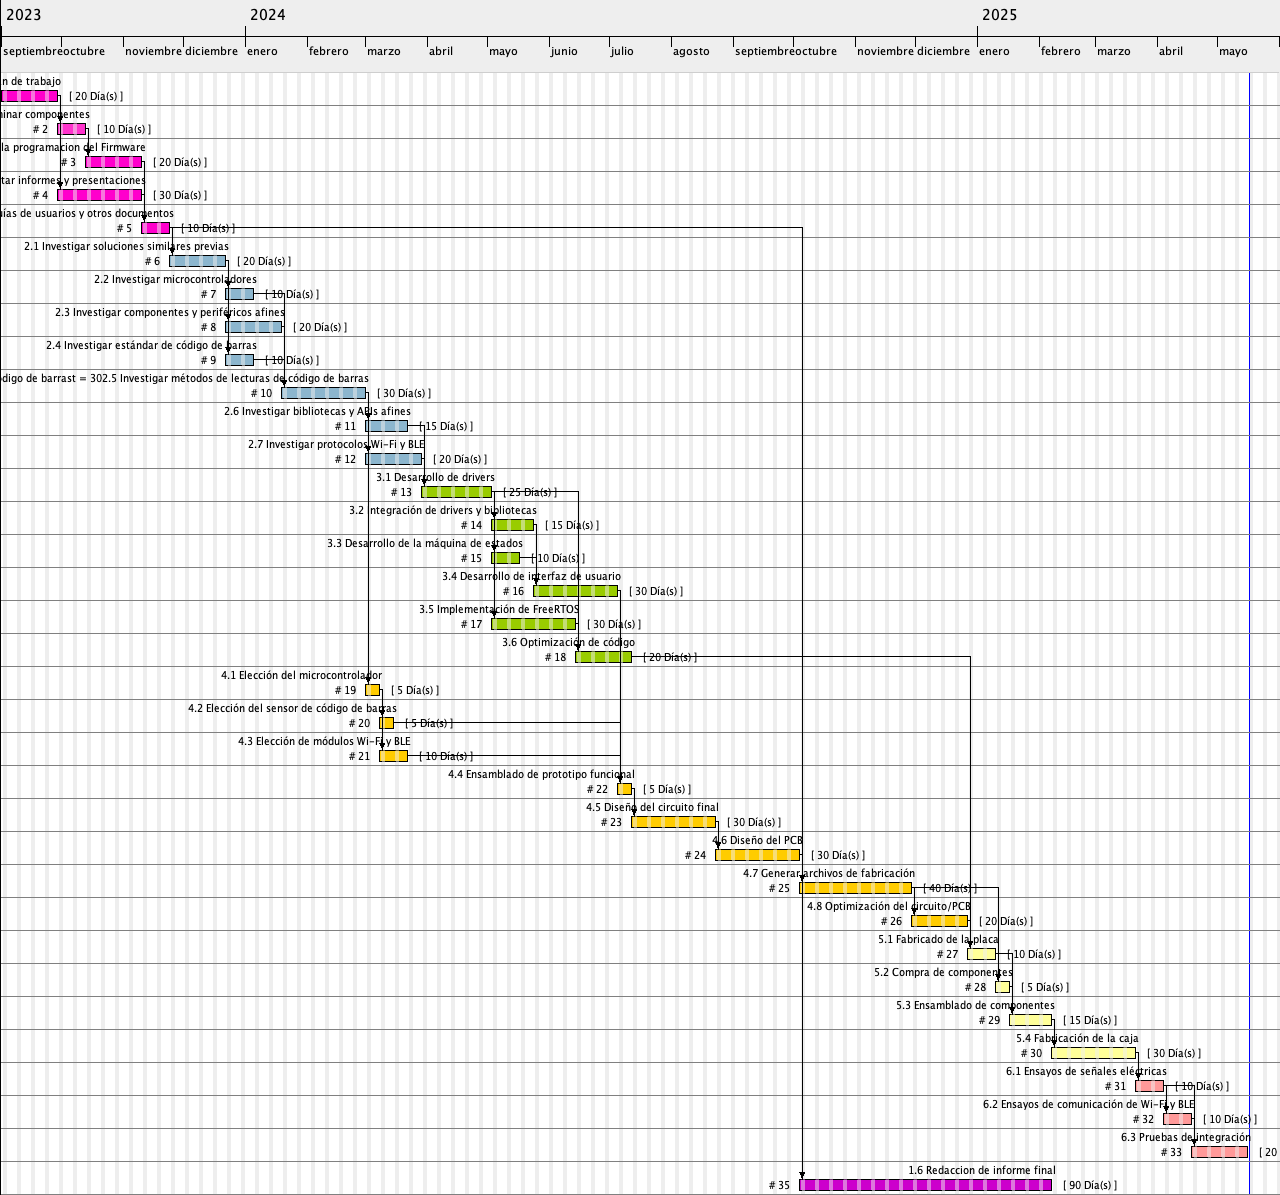
\includegraphics[width=26cm, height=17cm]{./Figuras/Gantt.png}
\caption{Diagrama de Gantt según la lista de tareas}
\label{fig:diagGantt}
\end{figure}

\end{landscape}



\section{12. Presupuesto detallado del proyecto}
\label{sec:presupuesto}

A continuación se listan todos los costos asociados al proyecto. Estos mismos están expresados en dólares americanos (USD).

\begin{table}[htpb]
\centering
\begin{tabularx}{\linewidth}{@{}|X|c|r|r|@{}}
\hline
\rowcolor[HTML]{C0C0C0} 
\multicolumn{4}{|c|}{\cellcolor[HTML]{C0C0C0}COSTOS DIRECTOS} \\ \hline
\rowcolor[HTML]{C0C0C0} 
Descripción &
  \multicolumn{1}{c|}{\cellcolor[HTML]{C0C0C0}Cantidad} &
  \multicolumn{1}{c|}{\cellcolor[HTML]{C0C0C0}Valor unitario} &
  \multicolumn{1}{c|}{\cellcolor[HTML]{C0C0C0}Valor total} \\ \hline
 Trabajo directo: horas de ingeniería & 
  \multicolumn{1}{c|}{612} &
  \multicolumn{1}{c|}{15 usd} &
  \multicolumn{1}{c|}{9180 usd} \\ \hline
Dispositivos de testing &
  \multicolumn{1}{c|}{1} &
  \multicolumn{1}{c|}{300 usd} &
  \multicolumn{1}{c|}{300 usd} \\ \hline
Componentes electrónicos &
  \multicolumn{1}{c|}{1} &
  \multicolumn{1}{c|}{500 usd} &
  \multicolumn{1}{c|}{500 usd} \\ \hline
Placas PCB &
  \multicolumn{1}{c|}{1} &
  \multicolumn{1}{c|}{50 usd} &
  \multicolumn{1}{c|}{50 usd} \\ \hline
Cajas y contenedores &
  \multicolumn{1}{c|}{1} &
  \multicolumn{1}{c|}{50 usd} &
  \multicolumn{1}{c|}{50 usd} \\ \hline

\multicolumn{3}{|c|}{SUBTOTAL} &
  \multicolumn{1}{c|}{10080 usd} \\ \hline
\rowcolor[HTML]{C0C0C0} 
\multicolumn{4}{|c|}{\cellcolor[HTML]{C0C0C0}COSTOS INDIRECTOS} \\ \hline
\rowcolor[HTML]{C0C0C0} 
Descripción &
  \multicolumn{1}{c|}{\cellcolor[HTML]{C0C0C0}Cantidad} &
  \multicolumn{1}{c|}{\cellcolor[HTML]{C0C0C0}Valor unitario} &
  \multicolumn{1}{c|}{\cellcolor[HTML]{C0C0C0}Valor total} \\ \hline

Administración &
  \multicolumn{1}{c|}{50} &
  \multicolumn{1}{c|}{2 usd} &
  \multicolumn{1}{c|}{100 usd} \\ \hline
  Horas de electricidad &
  \multicolumn{1}{c|}{670} &
  \multicolumn{1}{c|}{0,1 usd} &
  \multicolumn{1}{c|}{67,5 usd} \\ \hline
\multicolumn{3}{|c|}{SUBTOTAL} &
  \multicolumn{1}{c|}{167,5 usd} \\ \hline
\rowcolor[HTML]{C0C0C0}
\multicolumn{3}{|c|}{TOTAL} & 10247,5 usd
   \\ \hline
\end{tabularx}%
\end{table}


\section{13. Gestión de riesgos}
\label{sec:riesgos}

A continuación se listan los principales riesgos asociados al proyecto, junto con sus estimaciones de sus consecuencias:
 
Riesgo 1: Imposibilidad para cumplir los plazos del proyecto.
\begin{itemize}
	\item Severidad (S):8, retrasaría los plazos de entrega del proyecto, lo que intrínsecamente implica un costo adicional.\\
	\item Probabilidad de ocurrencia (O):7, además de ser un proyecto personal, todo el trabajo relacionado va a ser realizado por una única persona.\\
\end{itemize}   

Riesgo 2: Errores de diseño del prototipo
\begin{itemize}
	\item Severidad (S): 6, generaría retrasos e implicaría un costo mayor para el prototipo, producto de los reintentos.
	\item Ocurrencia (O): 5, si bien el prototipo es novedoso, los requerimientos no son excesivamente rigurosos.
\end{itemize}

Riesgo 3: Demora en la adquisición de componentes
\begin{itemize}
	\item Severidad (S):9 , existen pocas alternativas a los dispositivos que se requieren para realizar el proyecto, siendo el lector de código de barras indispensable e irreemplazable.
	\item Ocurrencia (O): 6, el contexto país no es tan favorable y presta a varios posibles problemas desde el envío del componente hasta la forma de pago.
\end{itemize}

Riesgo 4: Falta de documentación de los periféricos o bibliotecas a utilizar
\begin{itemize}
	\item Severidad (S):5 , al ser dispositivos/bibliotecas dedicadas, es posible que su documentación no sea clara
	\item Ocurrencia (O): 3, son dispositivos utilizados de forma masiva.
\end{itemize}

Riesgo 5: Problemas en el diseño de la interfaz gráfica.
\begin{itemize}
	\item Severidad (S):3 , no influye en el funcionamiento del prototipo, sino que es principalemte sería un encordio para los usuarios.
	\item Ocurrencia (O): 4, no se tienen requerimientos rigurosos respecto al diseño de la interfaz, sino a la funcionalidad que otorga.
\end{itemize}


A continuación podemos observar la tabla de gestión de riesgo:

\begin{table}[htpb]
\centering
\begin{tabularx}{\linewidth}{@{}|X|c|c|c|c|c|c|@{}}
\hline
\rowcolor[HTML]{C0C0C0} 
Riesgo & S & O & RPN & S* & O* & RPN* \\ \hline
      Imposibilidad para cumplir los plazos del proyecto. & 8  &  7 &  56  &   2 &  8  & 16     \\ \hline
      Errores de diseño del prototipo & 6  & 5  &  30   &   4 & 4   &16      \\ \hline
      Demora en la adquisición de componentes &  9 & 6  & 54    &    &    &      \\ \hline
      Falta de documentación de los periféricos o bibliotecas a utilizar &  5 & 3  &  15   &    &    &      \\ \hline
      Problemas en el diseño de la interfaz gráfica. &  3 & 4  &   12  &  4  &  6  &  24    \\ \hline
\end{tabularx}%
\end{table}

Criterio adoptado: 
Se tomarán medidas de mitigación en los riesgos cuyos números de RPN sean mayores o iguales a 30.
A continuación se lista el plan de mitigación para cada tarea
 
Riesgo 1: Planificar de forma adecuada el desarrollo del proyecto, dando tiempos de espera correctos para cada tarea.
  - Severidad (S):2 una correcta planificación mitiga los riesgos asociados a los tiempos de entrega.
  - Probabilidad de ocurrencia (O): 8 Requiere de mucha disciplina seguir un plan de forma concisa.

Riesgo 2: Se va a dividir el prototipo en módulos independientes, de forma tal de poder evaluar a cada uno por separado, siendo mas sencillo analizar y detectar errores en cada uno.
  - Severidad (S):4 Disminuye la complejidad del diseño.
  - Probabilidad de ocurrencia (O): 4 Al ser módulos mas pequeños, suelen ser más sencillos y suelen tener objetivos claros, haciendo más difícil equivocarse.
Riesgo 3: Se va a iniciar el proceso de adquisición de componentes lo más temprano posible, de forma tal de disponer de un mayor tiempo para que en caso de ser desfavorable, poder tomar otras medidas , como reemplazar el componente .
  - Severidad (S):4 Al tener una ventana de tiempo mayor (y eventualmente una mayor variedad de componentes) puedo ir almacenando los componentes a medida que son recibidos, lo que permite ir adelantando trabajo según los componentes que vayan arribando.
  - Probabilidad de ocurrencia (O): 6 Una cantidad de elementos mayo supone una mayor probabilidad, ya que aumenta la posibilidad de que al menos un componente se demore.



\section{14. Gestión de la calidad}
\label{sec:calidad}


A continuación  se listan los principales requerimientos del proyecto, junto con sus acciones de verificación y validación para cada uno:

\begin{itemize} 
\item Req \#2.1: El módulo deberá alimentarse a través de una batería.

\begin{itemize}
	\item Se verificarán las diferentes especificaciones de las distintas baterías disponible en el mercado, para adecuar el dispositivo a cada una.
	\item Se medirá el consumo energético mediante un multímetro, para que la batería no se agote de forma acelerada.   
\end{itemize}


\item Req \#2.2: El módulo deberá poder comunicarse mediante el estándar IEEE 802.11 b/g/n.

\begin{itemize}
	\item Se verificará que el periférico seleccionado cuente con las capacidades para realizar el estándar según lo indica la documentación de la norma vigente.
	\item Se validará que el dispositivo pueda enviar paquetes de datos a través de esta vía.  
\end{itemize}

\item Req \#2.3: El módulo deberá poder comunicarse utilizando Bluetooth Low Energy.

\begin{itemize}
	\item Se verificará la documentación de la norma, para adecuar el dispositivo y su consumo energético a la norma.
	\item Se validará que el dispositivo pueda conectarse de forma sostenida con un dispositivo móvil a través de bluetooth. 
\end{itemize}


\item Req \#2.5: El módulo deberá comunicarse vía API a la red para identificar el producto.

\begin{itemize}
	\item Se verificará la documentación del servicio, junto con la especificación del lector para extraer el código de forma exitosa.
	\item Se validará que efectivamente por cada escaneo se reconozca de forma efectiva el producto. 
\end{itemize}


\item Req \#2.6: El módulo deberá detectar los códigos de barras mediante un lector apropiado o cámara fotográfica.

\begin{itemize}
	\item Se verificarán los requisitos por el periférico para poder garantizar una lectura de código de forma exitosa en diferentes condiciones de iluminación, para así favorecer la versatilidad.
	\item Se validará que el dispositivo sea capaz de detectar y leer códigos de forma exitosa en diferentes situaciones con diferentes intensidades de luz.
\end{itemize}

\item Req \#3.2: Se realizarán tests de forma independiente para cada módulo, y de integración para cada una de las funcionalidades del mismo.

\begin{itemize}
	\item Se verificarán las especificaciones técnicas necesarias para cada módulo, de forma de lograr funcionalidades independientes para cada parte.
	\item Se validará que cada módulo tenga su esquema de pruebas, para que cada uno garantice la funcionalidad independiente del prototipo integral.
\end{itemize}

\item Req \#3.3: El firmware deberá priorizar el ahorro energético.

\begin{itemize}
	\item Se verificará la documentación del microprocesador, de forma tal de optimizar el manejo energético a lo largo del código.
	\item Se validará su consumo medio, mediante la medición de la corriente que consume el módulo.
\end{itemize}

\item Req \#1.3: El sistema debe llevar a cabo un conteo de los objetos que ingresan y/o egresan.

\begin{itemize}
	\item Se verificará que el dispositivo sea capaz de que una vez identificado el objeto, entienda la acción que ocurrió (se agregó o se sacó) y en base a eso actualice el stock.
	\item Se validará mediante la repetición de ingresos y egresos para un número determinado de objetos.
\end{itemize}

\item Req \#1.4: El sistema almacenará el inventario de forma local.

\begin{itemize}
	\item Se verificará que la cantidad de objetos detectados proveniente de la API, coincida con la cantidad de códigos almacenados.
	\item Se validará el conteo mediante la inspección de la memoria en tiempo de ejecución del código.
\end{itemize}



\end{itemize}


\section{15. Procesos de cierre}    
\label{sec:cierre}

A continuación se establecen las pautas para realizar la evaluación final del proyecto, contemplando las siguientes actividades:

\begin{itemize}
	\item Pautas de trabajo que se seguirán para analizar si se respetó el Plan de Proyecto original, a cargo de \authorname:\\
	 - Evaluación de las tareas y los tiempos: se confexionará una tabla en la cual se compararán las tareas propuestas con las realizadas y los tiempos propuestos frente a los reales. Se calcularán los desvíos, identificando sus principales causas.\\
  - Evaluación de costos: Se realizará una comparación entre los costos estimados frente a los costos resultantes luego de terminar el proyecto, de forma tal de que en caso de existir diferencias, identificar el porqué.
	\item Identificación de las técnicas y procedimientos útiles e inútiles que se emplearon, y los problemas que surgieron y cómo se solucionaron:
	 - \authorname será el encargado de realizar  un informe identificando las técnicas y procedimientos que hayan resultado beneficiosos como perjudiciales para el desarrollo del proyecto.
	\item Se invitará a la presentación del proyecto final a todas aquellas personas que hayan contribuido en alguna forma con el  proyecto. Allí se agradecerá al director y del proyecto, a jurados, compañeros, docentes y autoridades de la Carrera de Especialización en Sistemas Embebidos.
\end{itemize}



\end{document}
